\appendix

\section{Evaluation of the redshift distribution}
\label{sec:moments}
%(Alex Malz)

Perhaps the most popular application of \pzpdf s is the estimation of the overall redshift distribution $N(z)$, a quantity that enters some cosmological calculations and the true value of which is known for the DC1 data set and will be denoted as $\tilde{N}(z)$.
In terms of the prior information provided to each method, the true redshift distribution satisfies the tautology $\tilde{N}(z) = p(z \vert I_{D})$ due to our experimental set-up; because the DC1 training and template sets are representative and complete, $I_{D}$ represents a prior that is also equal to the truth.
In this ideal case of complete and representative prior information, the method that would give the best approximation to $\hat{N}(z)$ would be one that neglects all the information contained in the photometry $\{d_{i}\}_{N_{tot}}$ and gives every galaxy the same \pzpdf\ $\hat{p}_{i}(z) = \tilde{N}(z)$ for all $i$; the inclusion of any information from the photometry would only introduce noise to the optimal result of returning the prior.
This is the exact estimator, \trainz, that we have described in Section~\ref{sec:trainz}, and which will serve as an experimental control.

\subsection{Metrics of the stacked estimator of the redshift distribution}
\label{sec:stackedmetrics}

Though alternatives exist \citep{Malz:chippr}, ``stacking'' according to
\begin{equation}
  \label{eq:stacked}
  \hat{N}^{H}(z) \equiv \frac{1}{N_{tot}}\ \sum_{i}^{N_{tot}}\ \hat{p}^{H}_{i}(z)
\end{equation}
is the most widely accepted method for obtaining $\hat{N}^{H}(z)$ as an estimator of the redshift distribution from \pzpdf s derived by a method $H$.
Though we do not endorse the use of the stacked estimator of the redshift distribution, we use it under the untested assumption that the response of our metrics of $\hat{N}^{H}(z)$ will be analogous to the same metrics applied to a principled estimator of the redshift distribution.
In addition, very few scientific use cases will employ the overall $\hat{N}(z)$ with no cuts, as we explore in this paper.
We discuss in Section~\ref{sec:futurework} variants of the stacked estimator, such as realistic tomographic binning schemes, that will be explored in future work.

As $N(z)$ is itself a univariate PDF, we apply the metrics of the previous sections to it as well.
We additionaly calculate the first three moments
\begin{equation}
  \label{eq:moment}
  \langle z^{m}\rangle \equiv \int_{-\infty}^{\infty} z^{m} N(z) dz
\end{equation}
of the estimated redshift distribution $\hat{N}^{H}(z)$ for each code and compare them to the moments of the true redshift distribution $\tilde{N}(z)$.
Under the assumption that the stacked estimator is unbiased, a superior method minimizes the difference between the true and estimated moments.

\subsection{Performance on the stacked estimator of the redshift distribution}
\label{sec:stackedmetrics_results}

Figure~\ref{fig:nz} shows the stacked estimator $\hat{N}(z)$ of the redshift distribution for each code compared to the true redshift distribution $\tilde{N}(z)$, where the stacked estimator has been smoothed for each code in the plot using a kernel density estimate (KDE) with a bandwidth chosen by Scott's Rule \citep{Scott:1992} in order to minimize visual differences in small-scale features; the quantiative statistics, however, are calculated using the empirical CDF which is not smoothed.

\begin{figure*}
\centering
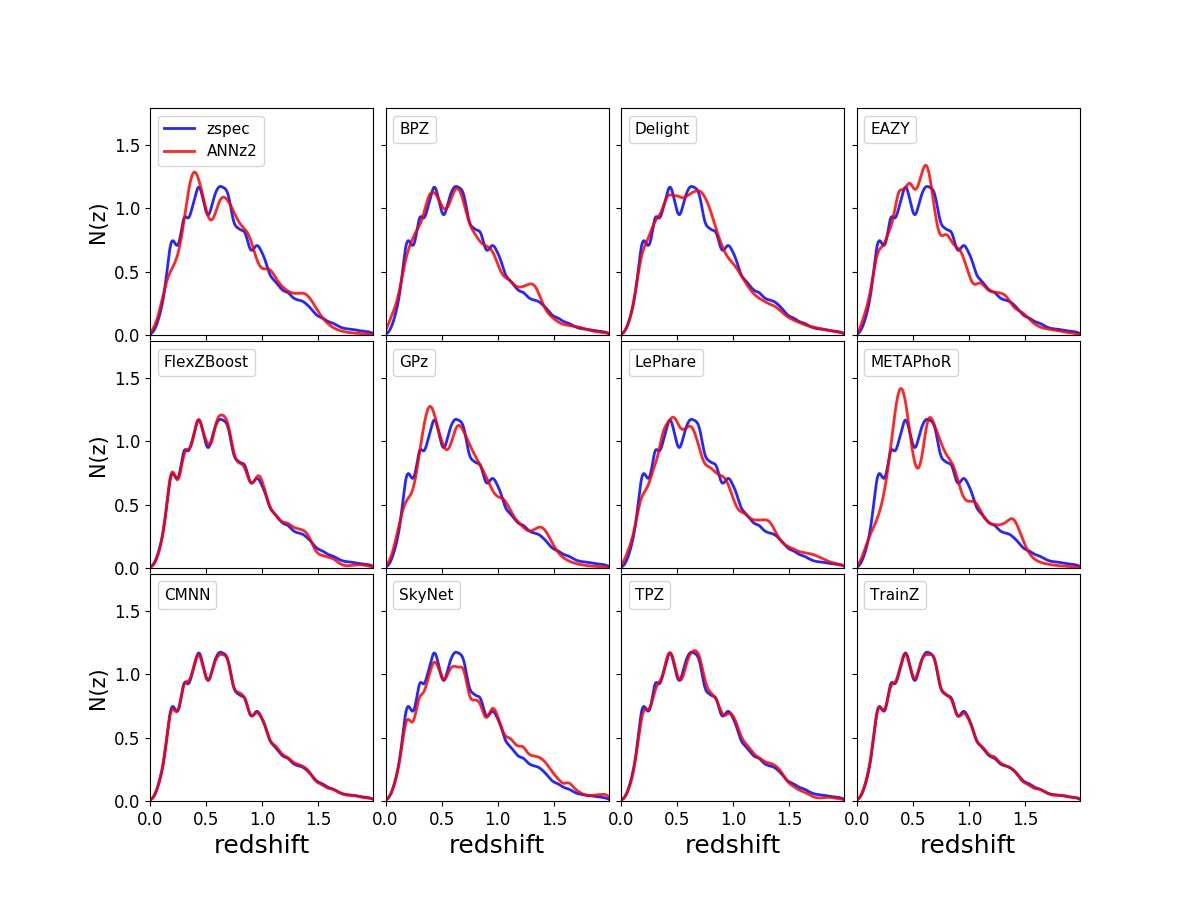
\includegraphics[width=0.74\textwidth]{fig/NZsumplot_12codes_scottsrule.jpg}
\caption{The smoothed stacked estimator $\hat{N}(z)$ of the redshift distribution (red) produced by each code (panels) compared to the true redshift distribution $\tilde{N}(z)$ (blue).
Varying levels of agreement are seen among the codes, with the smallest deviations for \cmnn, \flexzboost, \tpz, and \trainz.}
\label{fig:nz}
%\aim{Arguably this could also be clarified by showing the true $n'(z)$ once and then differences from it for each cod's stacked estimator\dots}\scc{what if we plot the difference between true and stacked rather than soverposing the two lines? Sam please do not hate me.}
\end{figure*}

Many of the codes, including all the model-fitting approaches and \annz, \gpz, \metaphor, and \skynet\ from the data-driven camp, overestimate the redshift density at $z \sim 1.4$.
This behavior is a consequence of the $4000\ {\rm \AA}$ break passing through the gap between the $z$ and $y$ filters, which induces a genuine discontinuity in the $z - y$ colour as a function of redshift that can sway the \pzpdf\ estimates in the absence of bluer spectral features.

\annz, \gpz, and \metaphor\ show signs of overtraining, estimating enhanced peaks and diminished troughs relative to the training set, an obstacle that may be overcome with adjustment of the implementation.

As expected, \trainz\ perfectly recovers the true redshift distribution: as the training sample is selected from the same underlying distribution as the test set, the redshift distributions are identical, up to Poisson fluctuations due to the finite number of sample galaxies.
\cmnn\ is also in excellent agreement for similar reasons: with a representative training sample of galaxies spanning the colour-space, the sum of the colour-matched neighbour redshifts should return the true redshift distribution.
\flexzboost\ and \tpz\ also perform superb recovery of the true redshift distribution, with only a slight deviation at $z \sim 1.4$.
Our metrics, however, cannot discern whether these four approaches, as well as \delight, are spared the $z \sim 1.4$ degeneracy in $\hat{N}(z)$ because they have more effectively used information in the data or if the impact is simply washed out by the stacked estimator's effective average over the test set galaxy sample.
See Appendix~\ref{sec:pointmetrics} for further discussion of the $z \sim 1.4$ issue.

Figure~\ref{fig:nz_stats} shows the quantitative Kolmogorov-Smirnoff (KS), Cramer-Von Mises (CvM), and Anderson Darling (AD) test statistics for each of the codes for the $\hat{N}(z)$ based measures.
%\red{Can p-values be supplied for each statistic? The statistics themselves are difficult to interpret, other than ``lower is better'' (no, p-values are very difficult to compute for non-uniform distributions)}
The stacked estimators of the redshift distribution for \cmnn\ and \trainz\ best estimate $\tilde{N}(z)$ under these metrics, and the only codes that do especially poorly are \eazy, \lephare, \metaphor, and \skynet.
It is unsurprising that \cmnn\ scores well, as with a near perfectly representative training set means that choosing neighbouring points in color/magnitude space should lead to excellent agreement in the final $\hat{N}(z)$ estimate.

\begin{figure*}
\centering
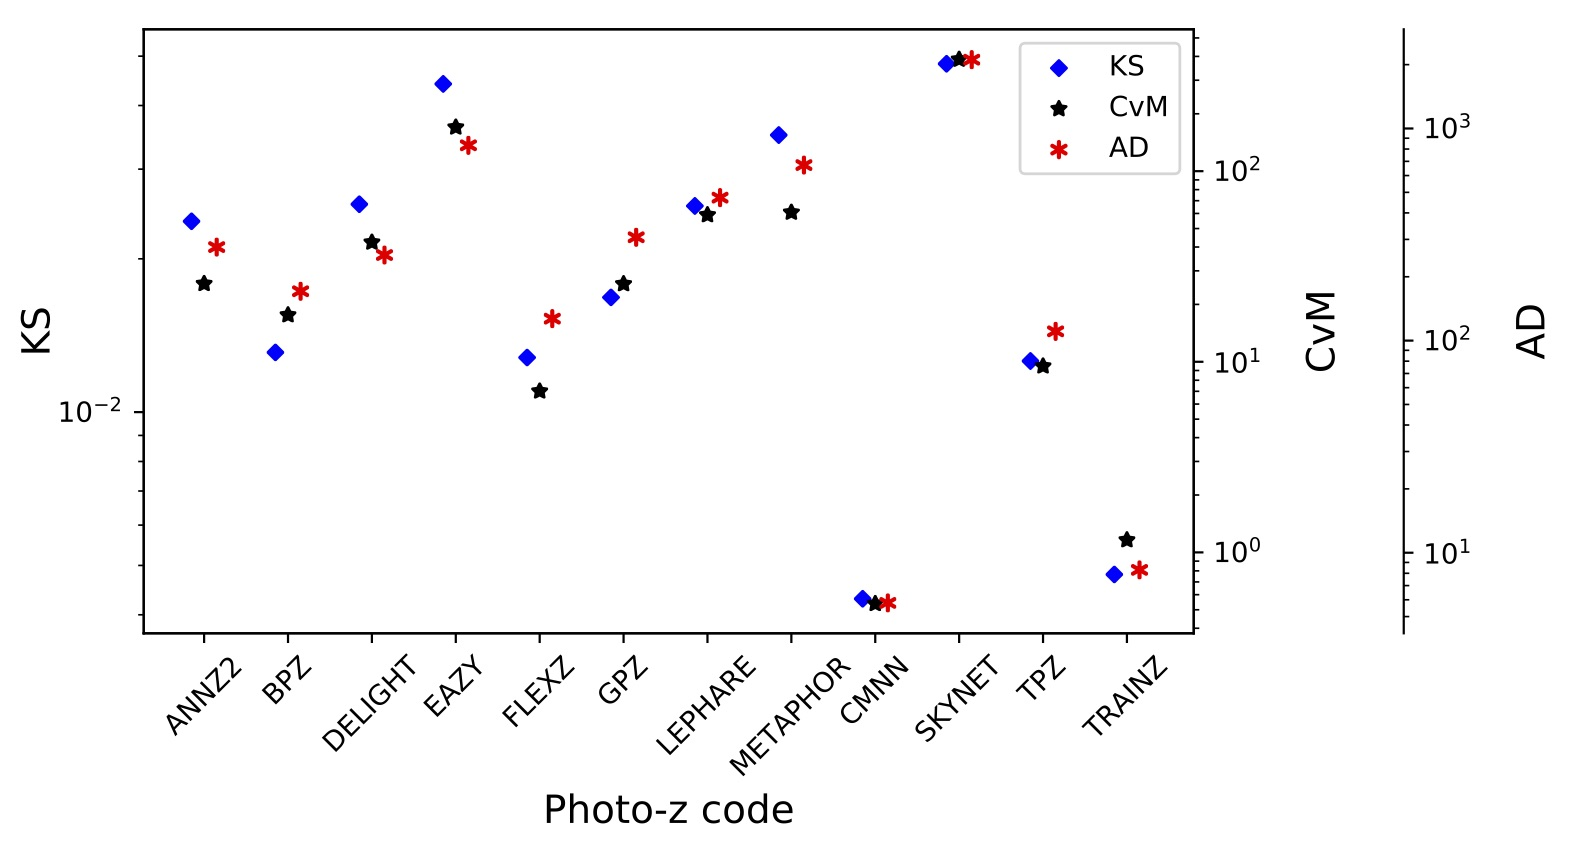
\includegraphics[width=0.74\textwidth]{fig/KSvsCvMvsAD_NZ_withnull_jpg.jpg}
\caption{A visualization of the Kolmogorov-Smirnoff (KS, blue diamond), Cramer-von Mises (CvM, black star), and Anderson-Darling (AD, red asterisk) statistics for the $\hat{N}(z)$ distributions.
We make the reassuring observation that these related statistics do not disagree significantly with one another.
\cmnn\ performs comparably well to \trainz, the control case, while \skynet\ scores poorly due to an overall bias in its redshift predictions.}
\label{fig:nz_stats}
\end{figure*}

It is, however, surprising that \tpz\ does well on $\hat{N}(z)$ given its poor performance on the ensemble \pzpdf s, especially knowing that \tpz\ was optimized for \pzpdf\ ensemble metrics rather than the stacked estimator of the redshift distribution.
A possible explanation is the choice of smoothing parameter chosen during validation, which affects \pzpdf\ widths as well as overall redshift bias and could be modified to improve performance under the \pzpdf\ metrics.

The first three moments of the stacked $\hat{N}(z)$ distribution relative to the empirical estimate of the truth distribution are given in Table~\ref{tab:moments}.
Accuracy of the moments varies widely between codes, raising concerns about the propagation to cosmological analyses.
%\red{[mention that we are calculating moments for the entire sample, will look at fiducial tomographic bins in a follow-up paper (unless group and reviewers realy think we should include in this paper.]}
%\red{FlexZBoost has some of the best $n(z)$ statistics, but the moments are not good.  Why is this?  Is it the over/underprediction of the high redshift part of the distribution?  Discuss this after talking with Rafael.}

\begin{table}
\setlength{\tabcolsep}{2pt}
\caption{Moments of the stacked estimator $\hat{N}(z)$ of the redshift distribution.
Most of the codes considered recover the moments of $\tilde{N}(z)$}
\label{tab:moments}
\begin{tabular}{lccc}
\hline
\hline
 \multicolumn{4}{l}{Moments of $\hat{N}(z)$} \\
\hline
Estimator  & mean       & variance    & skewness \\
Empirical ``truth'' & 0.701 & 0.630 & 0.671  \\
\hline
\annz       & 0.702      & 0.625      & 0.653    \\
\bpz        & 0.699      & 0.629      & 0.671    \\
\delight    & 0.692      & 0.609      & 0.638    \\
\eazy       & 0.681      & 0.595      & 0.619    \\
\flexzboost & 0.694      & 0.610      & 0.631    \\
\gpz        & 0.696      & 0.615      & 0.639    \\
\lephare    & 0.718      & 0.668      & 0.741    \\
\metaphor   & 0.705      & 0.628      & 0.657    \\
\cmnn       & 0.701      & 0.628      & 0.667    \\
\skynet     & 0.743      & 0.708      & 0.797    \\
\tpz        & 0.700      & 0.619      & 0.643    \\
\hline
\trainz	    & 0.699 		 & 0.627 	    & 0.666 \\
\end{tabular}
\end{table}

\skynet\ exhibits redshift bias in Figure~\ref{fig:nz} and is a clear outlier in the first moment of $\hat{N}(z)$ in Table~\ref{tab:moments}.
The \skynet\ algorithm employs a random subsampling of the training set without testing that the subset is representative of the full population, and the implementation used here does not upweight rarer low- and high-redshift galaxies, as in \citet{Bonnett:15}, suggesting a possible cause that may be addressed in future work.

\section{\Pz\ point estimation and metrics}
\label{sec:pointmetrics}

While we assume that all science analysis will use full PDF information and do not recommend the use of single point estimates of redshift for most science applications, we include a brief evaulation as an Appendix.
Plots of the point estimates can be a useful qualitative diagnostic of photo-z code performance, i.~e.~examining point photo-$z$ vs.~spec-$z$ plots visually can give a quick impression of some common trends in different codes.
Computing point estimate statistics may also be useful for more direct historical comparisons from older photo-z evaluations.
If a point-estimate is preferred for a specific science case, it is fairly simple to compute the mean, mode, or some other simple estimator from each $p(z)$, so these point estimates can be easily derived from the stored $p(z)$.

\subsection{Reduction of \pzpdf s to point estimates}
\label{sec:pointest}

There are several common point estimators of photo-$z$ posteriors employed by different codes, e.~g. the mode, mean, median of the $p(z)$ distribution.
In addition, many of the machine learning based estimators can be set up to return a single redshift solution.
For example, \skynet\ can be configured to run as a regressor that returns a single float rather than a classifier that returns a 200-bin $p(z)$ estimate.
The single value returned by a machine learning based code may not correspond to a particular measure such as the mode or mean, and so to avoid interpretation of results that might be introduced by variations in choice of specific point-estimate implementation per code, we discard the code-specific point estimates.
We instead calculate point estimates more uniformly across the codes directly from the $p(z)$ using two measures, $z_{PEAK}$ and $z_{WEIGHT}$.
$z_{PEAK}$  is simply the maximum value attained for each galaxy p(z), the mode of the probability distribution.
$z_{WEIGHT}$ is defined similarly to how it is defined in \citet{Dahlen:13}, as the weighted mean of the redshift over the {\it main peak} of $p(z)$ containing the $z_{PEAK}$ value.
The main peak is defined by subtracting 0.05$\,\times\,z_{PEAK}$ from $p(z)$ and identifying the roots to isolate the peak containing $z_{PEAK}$, $z_{WEIGHT}$ is defined as the weighted mean redshift within this peak.
We restrict to a single peak in order to avoid confusion from bimodal and multimodal $p(z)$ such as those shown in bottom panels of Figure~\ref{fig:pz_examples}.
For example, for a bimodal probability distribution a weighted mean calculated over both peaks would fall between the peaks, at a redshift where the probability is minimal.
Restricting the weighting to a single peak ensures that the point estimate will fall in the region of maximum redshift probability.
%\red{Have Dritan check zweight description to make sure this is what was done.}
% The most common point estimators of photo-$z$ PDFs are the mode, median, and mean of the distribution.  Following \cite{Tanaka:17}, we report the values of the following metrics using whichever of these point estimators performs best for each method, noting which point reduction is used in each case.
%
\subsection{Metrics of \pz\ point estimates}
\label{sec:point_metrics}

We calculate the commonly used point estimate metrics of the overall photo-$z$ scatter ($\sigma_{z}$, the standard deviation of the photo-$z$ residuals), bias, and ``catastrophic outlier rate''.
Specifically, we calculate the metrics as follows:
we define $e_{z}$ as
\begin{equation}
e_{z} = \frac{z_{P} -z_{S}}{1+z_{S}}
\end{equation}
where $z_{P}$ is the point estimate and $z_{S}$ is the true redshift.
In practice, because the standard deviation calculation is quite sensitive to the outliers, we define the photo-$z$ scatter, $\sigma$ in terms of the Interquartile Range (IQR), the difference between the 75th and 25th percentiles of the $e_{z}$ distribution.
In order to match the usual meaning of a 1$\sigma$ interval, we scale the IQR and define $\sigma_{IQR} = IQR/1.349$, as there is a factor of 1.349 difference between the IQR and the standard deviation of a Normal distribution.
%$\sigma_{z}$ is, in practice, defined in terms the Interquartile Range (IQR) of $e_{z}$ values as $IQR/1.349$, where $IQR$ is the difference between the 75th and 25th percentiles of the $e_{z}$ distribution.  The factor of 1.349 relates the IQR of a Normal distribution to the standard 68\% range of a one $\sigma$ uncertainty.
%\scc{usually the statistical indicator defined as $\sigma$ is the standard deviation I know that is not a rule but if someone skips the test and go directly to the table (and we all know that a lot of people skips the definition of statistical indicator) could be confusing, could we report it as $\frac{IQR(e_z)}{1.349}$ or $\sigma_{IQR}$ that should be clear without any risk of confusion?}\red{Using IQR is done because IQR is less sensitive to outliers than calculating a sigma.  I've rewritten the text explaining this above.--SJS}
While many other studies define the bias based on the {\it mean} offset between true and estimated redshift, in this study we define the bias as the median value of $e_{z}$ for the sample.
We use median as it is, once again, less sensitive to outliers than the mean.
The catastrophic outlier fraction is defined as the fraction of galaxies with $e_{z}$ greater than the {\it larger} of $3\sigma_{IQR}$ or 0.06, i.e. 3$\sigma$ outliers with a floor of $\sigma_{IQR}$=0.02.
%\scc{again, is clearly not a rule but a huge number of paper refers to the mean as bias, could we use the word median, which is clear without any doubt rather than bias?}
%\red{I also have code to calculate $\sigma_{MAD}$, should we include this as well?  It's almost always within a few thousandths of $\sigma_{IQR}$, so I left it out for now}.
%\scc{we may just say that the two indicators reports almost the same value therefore there is no need for both of them?}
For reference, the goals stated in Section 3.8 of the LSST Science Book \citep{Abell:09} for photo-$z$ performance in these metrics, assuming perfect training knowledge (as we are testing in this paper) are:
\begin{itemize}
\item RMS scatter$ < 0.02(1+z)$
%\scc{actually the SB reports in page 75 that the goal of 0.02 is for the RMS of $\frac{\sigma_{z}}{(1+z)}$ while we are using IQR}
\item bias $<$ 0.003 %\scc{in page 518 of the SB is clearly reported that the mean is expected to be less than 0.003 in our case we have defined as bias the median and not the mean }
\item catastrophic outlier rate $<$ 10\% %\scc{clearly the number of outliers since are defined above $3\sigma$ strictly depends on the sigma definition, in the science book it seems to refer to the RMS of the $e_z$ distribution even ef it could be the standard deviation, but again I don't think it refers to IQR, therefore we could not consider exactly this numbers as reference.}
%\red{I am going off of conversations with Zeljko and how we {\it actually} computed the metrics in the Science Book (I have the scripts).  You are correct that several of these are slightly different than actually stated in the Science Book, or where the Science Book does not use very precise language as to what was done to compute the RMS or define the bias.  We can also cut out those specifics, or maybe say Ivezic private communication, maybe?  Also $\sigma_{z}$ defined in terms of IQR is exactly equivalent to the standard deviation when scaled by 1.349 for a Gaussian distribution, so the numbers are appropriate to cite in this context.  IQR is just a more robust way of calculating sigma for a distribution with outliers.--SJS }
%\scc{I am very sorry I am not saying that IQR is not fine, I want to keep the IQR my concerns are related to the notation and the \textit{reader understanding}, if I wrote $\sigma$ somewhere in a table the reader will understand for sure that is the traditional standard deviation (a lot of people skips the indicators definition for the \textit{obvious} ones), I am suggesting to replace the notation $\sigma$ with the notation $\sigma_{IQR}$ (or something like this) to avoid any confusion, and also to change from $bias$ to $median$ for the same reason. I agree that say Ivezic private communication could be better.}
\end{itemize}
These definitions are similar, but not exactly the same, as the $\sigma_{IQR}$ and median bias calculated here, but are similar enough for qualitative comparisons to the LSST goals.

%Scatter: SRD $\sigma<0.02(1+z)$
%Catastrophic Outler Rate: SRD $3\sigma$ ``catastrophic outlier'' rate below 10 per cent
%Bias: SRD bias$<0.003$

\subsection{Comparison of \pz\ point estimate metrics}
\label{sec:pointmetrics_results}

\begin{figure*}
\centering
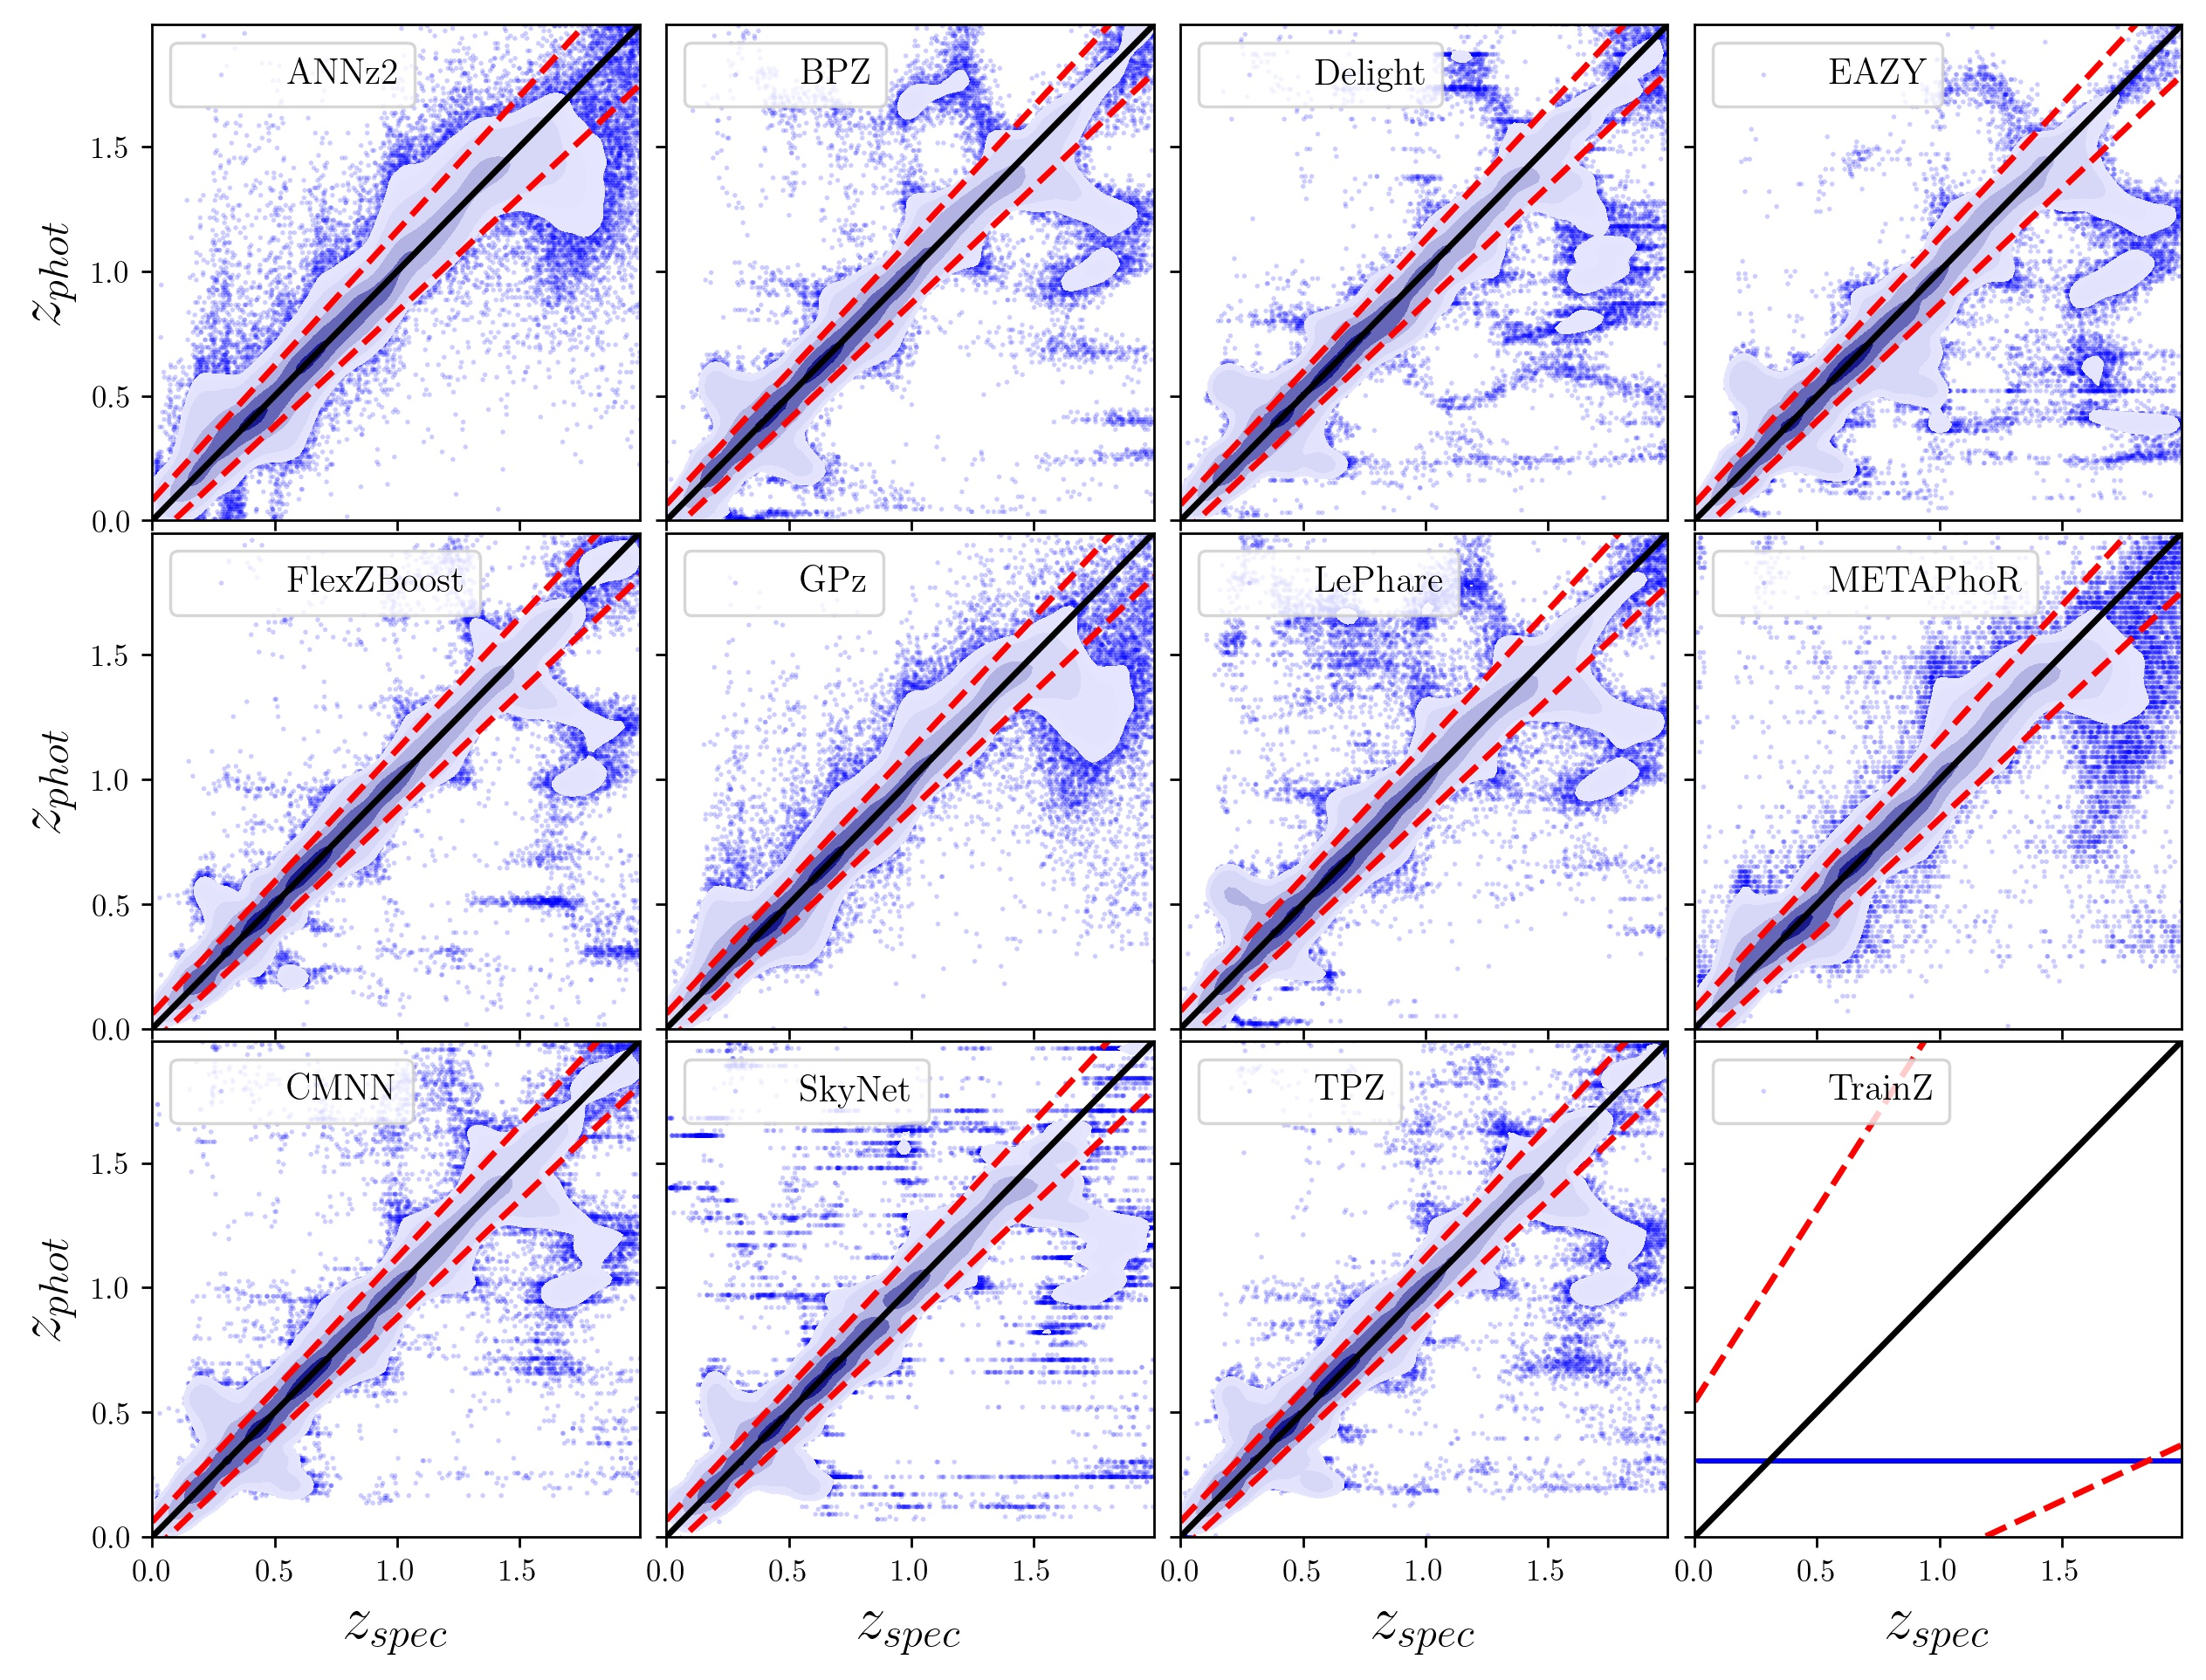
\includegraphics[width=0.49\textwidth]{fig/ZPEAK_szpz_threecolumn_12codes_navy_lowalpha.jpg}
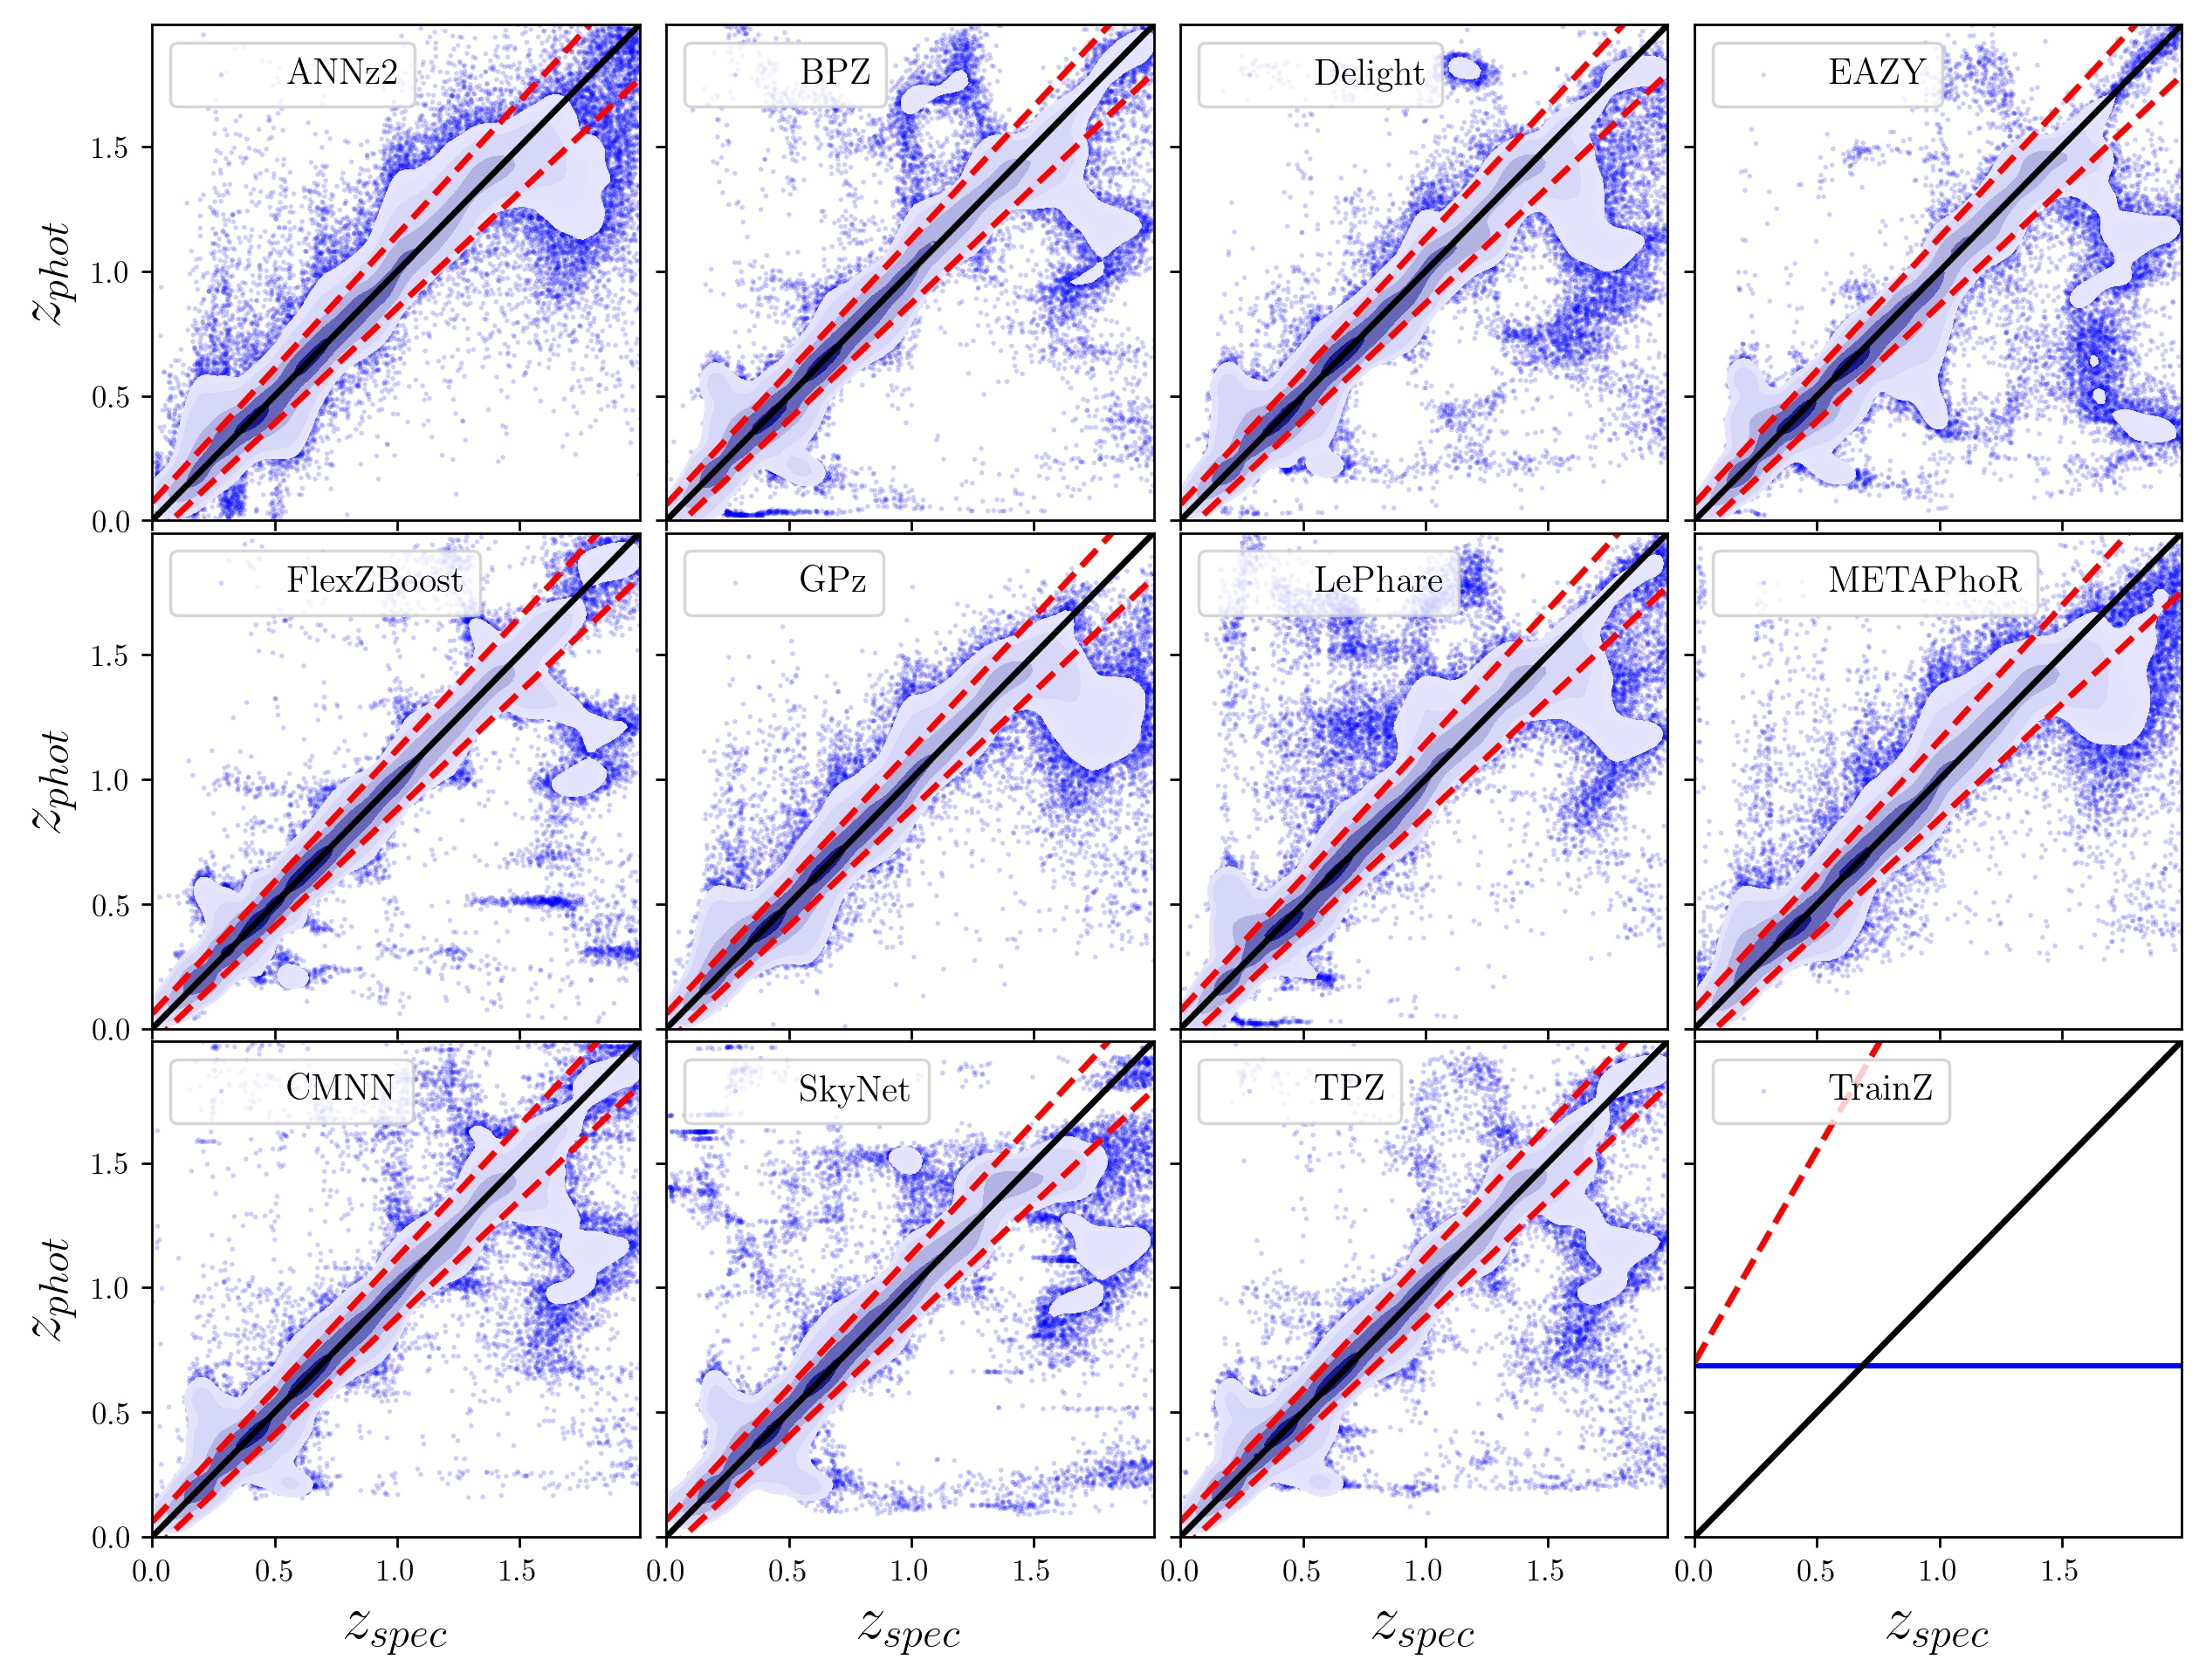
\includegraphics[width=0.49\textwidth]{fig/ZWEIGHT_szpz_threecolumn_12codes_navy_lowalpha.jpg}
\caption{\Pz\ point estimates reduced from the \pzpdf s, via the mode ($z_{PEAK}$, left panel) and mean ($z_{WEIGHT}$, right panel).
Point estimate density is represented with fixed density contours, while outliers at lower density are represented by blue points.
While use of point-estimate photo-$z$'s is not recommended, they do make for useful comparative and visual diagnostics.
In the lower-right panel of each plot, the \trainz\ estimator results in identical photo-$z$ estimates at the mode and mean of the training set $N'(z)$ distribution for all galaxies.}
\label{fig:pz_pointestimates}
\end{figure*}

Figure~\ref{fig:pz_pointestimates} shows the point estimates for both $z_{PEAK}$ and $z_{WEIGHT}$.
Point density is shown with mixed contours to emphasize that most of the galaxies do fall close to the $z_{phot}=z_{spec}$ line, while blue points show differing characteristics of the outlier populations.
The red dashed lines indicated the cutoff for catastrophic outliers, defined as: $max(0.06,3\sigma_{IQR})$.
As with the full $p(z)$ results, a variety of behaviours are evident in the different codes.  Table~\ref{tab:pointestimates} lists the scatter, bias, and catastrophic outlier fractions for the codes.
The performance of the codes for point metrics is highly correlated with performance on $p(z)$ based tests, which is to be expected, given that the point-estimates were derived from the $p(z)$.
Some discretization is evident in $z_{PEAK}$, particularly for \textsc{SkyNet}, due to the finite grid spacing of the reported $p(z)$.
These discreteness effects are mitigated by the weighting of $z_{WEIGHT}$, resulting in a smoother distribution of redshift estimates.
Several features perpendicular to the main $z_{phot}=z_{spec}$ line are evident.
These features are due to the 4000 angstrom break passing through the gaps between adjacent LSST filters.
These features are most prominent in template-based codes, but appear to some degree in all codes tested.

In even the best performing codes, there are visible occupied regions away from the $z_{phot}=z_{spec}$ line, corresponding to degenerate redshift solutions for certain LSST magnitudes and colors.
While use of the full information available via $p(z)$ mitigates their impact, a full understanding of the outlier population is critical for LSST science, particularly in tomographic applications %\red{I forget what exactly I was trying to say here, if someone else wants to take a crack at this it might be helpful --SJS}
%\scc{may be worth to say that the usage of further bands could mitigate this effect by removing the degeneration  usually induced from emission lines moving across different filters?}

\begin{table*}
\begin{center}
\caption{\Pz\ point estimate statistics}\label{tab:pointestimates}
\begin{tabular}{lcccccc}
\hline
\hline
                 &            & $Z_{PEAK}$  &          &  & $Z_{WEIGHT}$          &\\
\hline
\Pzpdf\ Code       & $\frac{\sigma_{IQR}}{(1+z)}$ & median  & \multicolumn{1}{|p{0.75cm}|}{\centering outlier \\fraction} & $\frac{\sigma_{IQR}}{(1+z)}$ & median & \multicolumn{1}{|p{0.75cm}|}{\centering outlier \\fraction}\\
\hline
\annz     & 0.0270  &  0.00063  & 0.044      & 0.0244  &  0.000307  & 0.047  \\
\bpz       & 0.0215  & -0.00175  & 0.035      & 0.0215  & -0.002005  & 0.032 \\
\delight   & 0.0212  & -0.00185  & 0.038      & 0.0216  & -0.002158  & 0.038 \\
\eazy      & 0.0225  & -0.00218  & 0.034      & 0.0226  & -0.003765  & 0.029 \\
\flexzboost& 0.0154  & -0.00027  & 0.020      & 0.0148  & -0.000211  & 0.017 \\
\gpz       & 0.0197  & -0.00000  & 0.052      & 0.0195  &  0.000113  & 0.051 \\
\lephare   & 0.0236  & -0.00161  & 0.058      & 0.0239  & -0.002007  & 0.056 \\
\metaphor  & 0.0264  &  0.00000  & 0.037      & 0.0262  &  0.001333  & 0.048 \\
\cmnn        & 0.0184  & -0.00132  & 0.035      & 0.0170  & -0.001049  & 0.034 \\
\skynet    & 0.0219  & -0.00167  & 0.036      & 0.0218  &  0.000174  & 0.037 \\
\tpz       & 0.0161  &  0.00309  & 0.033      & 0.0166  &  0.003048  & 0.031 \\
\hline
\trainz	   & 0.1808  &  -0.2086  & 0.000	  & 0.2335  & 0.022135  & 0.000\\
\end{tabular}
\end{center}
\end{table*}

Finally, we note that all twelve codes perform at or near the goals for point-estimates as outlined in the LSST Science Requirements Document\footnote{available at: \url{http://ls.st/srd}} and \citet{Graham:17}.
This is to be expected, given that the requirements were designed such that a point estimate photo-z would meet these requirements for perfect training data to a depth of $i<25$.
But, it is still an encouraging sign, given an updated mock galaxy simulation and the expanded set of photo-$z$ codes tested.
%\red{maybe say consistent with expectations, and a reference to Melissa's paper in here?  What else to say about nearly meeting point goals?}
